\documentclass[10pt,letterpaper]{article}

\usepackage{cogsci}
\usepackage{pslatex}
\usepackage{apacite}
\usepackage{amsmath}
\usepackage{float} 
\usepackage{graphicx}
\usepackage[skip=2pt]{caption}

%Comment out for submission
\cogscifinalcopy

\title{Rapid Presentation Rate Negatively Impacts the Contiguity Effect in Free Recall}
 
\author{{\large \bf Claudio Toro-Serey (ctoro@bu.edu) \and Ian M. Bright (imbright@bu.edu)} \\
  Department of Psychological and Brain Sciences, 64 Cummington Mall\\
  Boston, MA 02215 USA
  \AND
    {\large \bf Brad Wyble (bpw10@psu.edu)} \\
  Department of Psychology, 140 Moore Building\\
  University Park, PA 16801 USA
  \AND
  {\large \bf Marc W. Howard (marc777@bu.edu)} \\
  Department of Psychological and Brain Sciences, 64 Cummington Mall\\
  Boston, MA 02215 USA}


\begin{document}

\maketitle

\begin{abstract}
It is well-known that  in free recall participants tend to recall  
words presented close together in time in sequence, reflecting a form of
temporal binding.
This  contiguity effect is observed under many different experimental
conditions.  In order to understand the boundaries of the contiguity effect,
we measured the contiguity effect at presentation rates from
2~Hz (one word every 500~ms) to 8~Hz (one word every 125~ms). The contiguity
effect broke down as presentation rate increased.  This frequency matches the
upper bound of neural-related theta frequency, which has been linked to
temporal encoding of episodic memories. 
\textbf{Keywords:} 
Free recall, lag-CRP, contiguity effect 
\end{abstract}

\section{Introduction}

Cognitive neuroscientists have hypothesized that the successful retrieval of
an episodic memory is accompanied by a ``jump back in time,'' a recovery of
the previous memory's spatiotemporal context \cite{Tulv83}. In free recall
studies, this recovery manifests as the contiguity effect, wherein after the
successful recall of an item, the next item to be recalled is more likely to
be a close temporal neighbor than a more distant one \cite{Kaha96}. 
This distance is measured as lag, a directed distance between any two items in
a study list. For example, in the list ``absence, hollow, pupil, river,
darling'', the lag from absence to river is $+3$, while the lag from darling to
pupil is $-2$.  
In free recall studies the contiguity effect is typically asymmetric, such that
forward transitions are more likely to take place than backward transitions of
the same distance.  This effect is robust, appearing across a variety of
methodological manipulations \cite{Kaha12,HealKaha14}. 
For instance, the contiguity effect is observed with more or less the same
properties for lists of different modalities \cite{Kaha96}, when rehearsal is
discouraged \cite{HowaKaha99}, and when words are widely separated in time
\cite{HowaEtal08,Unsw08}.  \citeA{HealKaha14} noted that the contiguity effect
was observed for every individual participant in a large scale free recall
study.   Thus far, dramatic effects on the contiguity effect in free recall
have primarily been observed comparing patient populations; older adults and
memory disordered individuals show impaired contiguity effects
\cite{KahaEtal02,PaloEtal19}.
% The Palombo citation is:
%Medial temporal lobe amnesia is associated with a deficit in recovering
%temporal context 
%DJ Palombo, JM Di Lascio, MW Howard, M Verfaellie
%Journal of cognitive neuroscience 31 (2), 236-248


Beyond the contiguity effect, free recall contains many other well-explored
patterns of behavior. Individuals exhibit a strong recency effect during
immediate free recall tests \cite{GlanCuni66}. The primacy effect refers to
the well-known property that participants are more likely to recall items from
the beginning of a studied list \cite{Murd62}.   Both primacy and recency
effects are observed in the initiation of free recall \cite{Hoga75,Lami99};
primacy and recency are both robustly observed in the probability of first
recall,  a measure of the serial position curve considering only the first
recall.  The relative strength of primacy and recency  is not constant
\cite{Murd62}.  \citeA{DaveEtal05} found that presentation rates affect the
relative strength of primacy and recency, with primacy becoming more prevalent
as the presentation rate is increased.  They interpreted this as a consequence
of a failure for incoming items to enter a short-term store at very fast
presentation rates.

%Recency and primacy effects also manifest at the very beginning of recall.
%Individuals are more likely to begin recall at the beginning or end of a list,
%with a higher probability for more recent items \cite{HowaKaha99}. The effect
%of high presentation rates on the probability of first recall has yet to be
%reported. 

\nocite{DaveEtal05}
The ubiquity of the contiguity effect  in free recall presents something of a
theoretical problem.  If we knew the boundary conditions on the contiguity
effect it would presumably shed light on the processes supporting the binding
of experiences presented close together in time.  In this study we explore the
effects of increasing presentation rates on the contiguity effect.  If the
contiguity effect is disrupted at a particular rate, that suggests the time
scale over which the encoding processes necessary for temporal binding take
place.

Considerations from the ERP literature and rapid serial visual presentation
(RSVP) literature inform the time scale over which contiguity might be
disrupted.  A to-be-remembered stimulus typically evokes a P300 waveform
approximately 500~ms in duration that is thought to represent the updating of
memory representations, even when the stimulus duration itself is on the order
of 2 seconds \cite{Donc81}.
At presentation rates approaching 10~Hz, there is evidence that individual list
items are no longer processed as discrete items, and instead are merged into a
single extended cognitive event.  For example, individual items in 10~Hz lists
receive very low hit rates in an immediate recognition test even when the
stimuli are never-before-seen natural images \cite{PottLevy69}.  This poor
performance is in stark contrast to the excellent recognition memory for long
series of images  at slower rates of presentation \cite{Stan73,BradEtal08}.
However despite this lack of memorability, it is also clear that each item in
a 10~Hz stream is processed to some degree, since
it is possible to detect specific target items with highly probability
\cite{Pott76}.  If the processing of individual items in a list undergoes a
qualitative change as the presentation rate is increased to the point at which
the representations blend together, then the CRP and ratio of primacy and
recency may be abruptly altered. For example, the CRP effect may depend
on the ability to wrap individual list items in a discrete episodic
representation, and thus it may disappear with faster presentation rates. The
probability of first recall could also be altered, since a long-running stream of
rapidly presented items imposes a sequential cost on subsequent items due to
encoding interference from previous items \cite{WyblEtal09}.  


\section{Methods}

\subsection{Participants}

Three hundred thirty undergraduates from Syracuse University participated in
this study.  
Participants were excluded if they failed to recall a correct word in at least
one trial ($n = 15$), and if they did not perform all three conditions ($n =
7$). Data from 308 participants was used in subsequent analyses.  

\subsection{Procedure}

Participants took part in 18 trials. Each trial consisted of 20 words pulled from the Toronto Noun Pool \cite{FrieEtal82} 
Words were presented at three
presentations rates: 2~Hz, 4~Hz, and 8~Hz Participants completed six trials in
each condition. Trial order was randomized.  Participants were prompted to
verbally recall as many words as possible from the list. Responses were
recorded and later parsed using a semi-automatic speech parsing algorithm.

\subsection{Analysis}

We examined whether presentation rate affected either the average number of
valid recalls in a trial or median response latencies. This was done with a
repeated measures ANOVA. Post-hoc paired permutations (5000 iterations),
Cohen's D effect sizes on mean recalls, and median response latencies were then
performed to determine significant differences. Serial position curves (SPC),
were computed to show the overall probability of a word being recalled based
on its position in the list for each participant. We examined whether the recency
effect changed in relation to the primacy effect as a function of presentation
rate. We performed a mixed effects linear regression with subject as a mixed
effect and condition as fixed effect, in order to predict the difference in
the probability of recall for the first and last items in the list (i.e.,
probability for position 20 minus probability for position 1). 

PFR was calculated by dividing the number of times each position was recalled
by the total number of first recalls. We then averaged these probabilities
across participants per condition. Finally, we calculated the conditional
response probability (CRP) for each lag by dividing the number of correct
recall transitions at a given lag by the total number of possible correct
transitions at that lag. 
In order to control for serial position effects, which differed across
conditions, we restricted the lag-CRP analysis to transitions within the
middle of the list where probability of recall was approximately equal across
presentation rates.
In order to test for differences in the CRP at each
lag across conditions, we performed a number of mixed-effects logistic regressions. 
First, to examine the existence of contiguity effects at each rate,
we estimated the probability of recall based on absolute lag from the previously
recalled word for each presentation rate separately. Next, we estimated the full CRP as a function of the
interaction between the following fixed-effects predictors: absolute lag, its
direction (backwards or forwards from the previously recalled item), and 
presentation rate. We report Z- and T-scored coefficients for all
mixed-effects models.
%There is a tutorial at in the intro, but it can moved down here if thats more
%effective.

\section{Results}

\subsection{Rate Increments Produce Fewer but Faster Recalls}
%Alternate subsection title: As Presentation Rate Increases, fewer words are recalled but are recalled faster.

As shown in Figure~\ref{Descriptives}, the total number of words recalled
decreased as presentation rates increased (2~Hz: mean = 3.54, SD = 0.85; 4~Hz:
mean = 2.86, SD = 0.662; 8~Hz: mean = 2.41, SD = 0.62; ANOVA: $F(2, 614) =
309.2, p < 0.001$). Latencies also decreased as presentation rate increased 
(2~Hz: median = 1196 ms, SD = 517 ms; 4~Hz: median = 995 ms, SD = 401 ms; 8~Hz:
median = 910 ms, SD = 392 ms; ANOVA: $F(2, 614) = 61.38, p < 0.001$). Post-hoc
paired permutations confirmed these results, showing that the presentation
rate of 2~Hz yielded significantly higher number of recalls than 4~Hz ($p <
0.001$, Cohen's D $= 0.9$) and 8~Hz ($p < 0.001$, Cohen's D $= 1.5$), and that
4~Hz produced significantly more recalls than 8~Hz ($p < 0.001$, Cohen's D $=
0.69$). Similarly, overall recalls in the 2~Hz condition were significantly
slower than for 4~Hz ($p < 0.001$, Cohen's D $= 0.4$) and 8~Hz ($p < 0.001$,
Cohen's D $= 0.64$), with 8~Hz producing the fastest responses ($p < 0.001$,
Cohen's D $= 0.22$).   This is most likely attributable to the well-known
finding that in free recall interresponse time grows with output position
\cite{MurdOkad70}.

\begin{figure}
\begin{center}
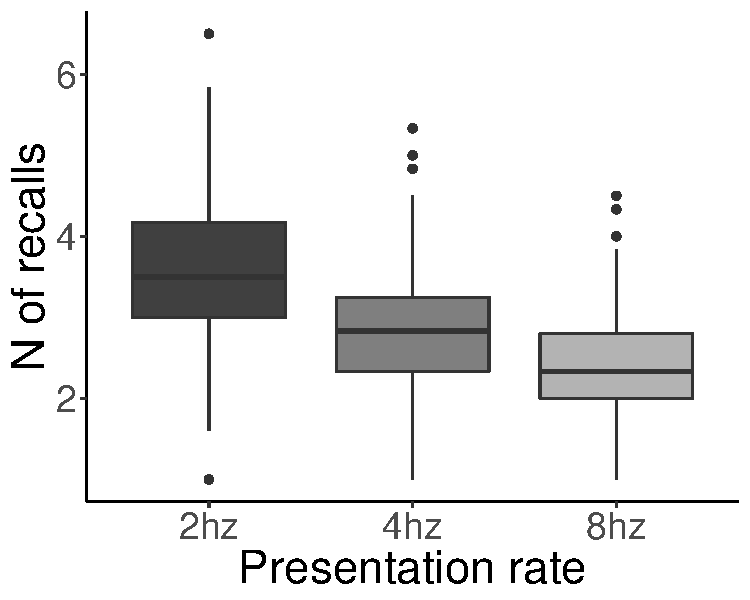
\includegraphics[width = .23\textwidth]{RSVPFR/recall_boxplot.pdf}
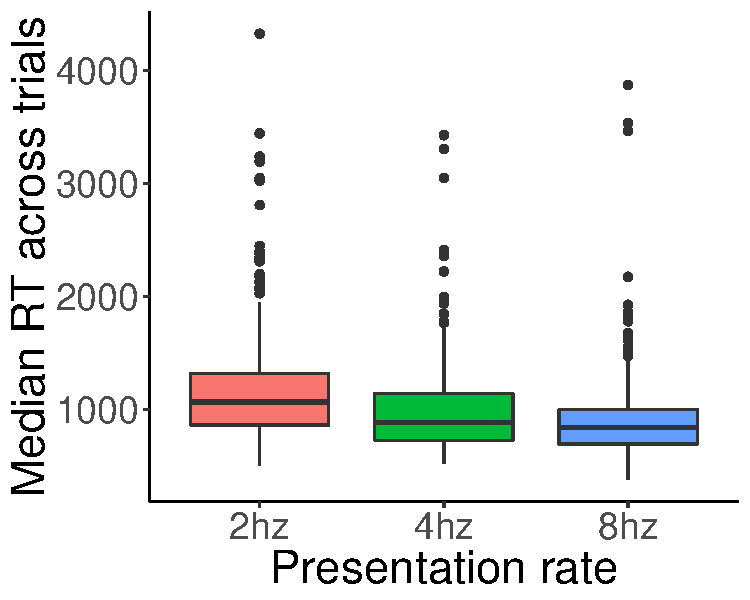
\includegraphics[width = .23\textwidth]{RSVPFR/rt_boxplot.pdf}
\end{center}
\caption{Left: Mean number of valid words recalled per trial across participants and presentation rates. The average number of recalled words decreased as presentation rate increased. Right: Median latencies (ms) across trials for each participant and presentation rate. Median latencies between valid recalls decreased as presentation rate increased} 
\label{Descriptives}
\end{figure}

\subsection{Increasing Presentation Rates Increases the Primacy Effect and Decreases the Recency Effect}
%Alternative: Primacy and Recency effects are inversely affected by presentation rate

Participants were more likely to begin recall by reporting a word at the
beginning or end of the list (Figure~\ref{PFR}). In agreement with our
hypothesis, as the presentation rate increased, the probability of first recall
shifted from showing a stronger recency effect to a stronger primacy effect.
This shift resulted in a flip such that the probability of first recall was
higher for the last item on the list than the first item for a 2~Hz
presentation rate, but lower in the 8~Hz condition.

\begin{figure}
\begin{center}
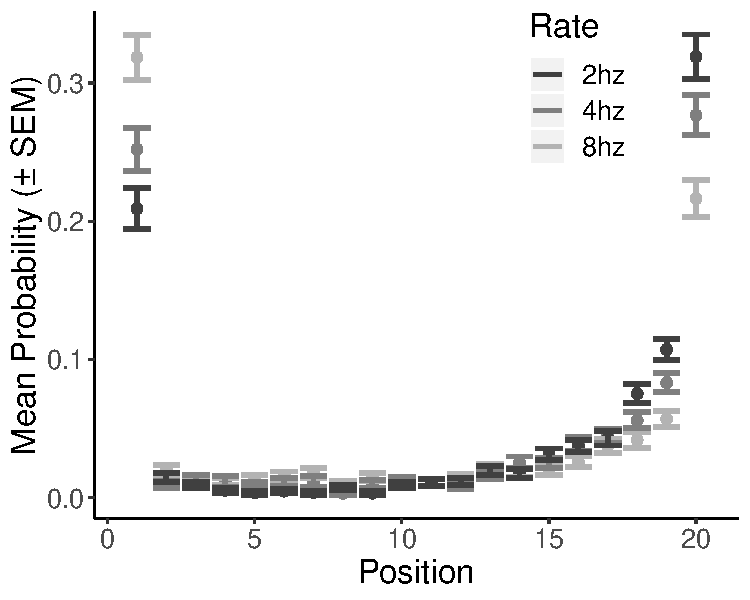
\includegraphics[width = .4\textwidth]{PFR_adjusted.pdf}
\end{center}
\caption{Probability of first recall. Participants tended to begin recall by
naming an item from the beginning or end of the list. At lower presentation
rates, participants showed a tendency to start recall at the end of the list
rather than the beginning, but this tendency flipped for high presentation
rates.} \label{PFR}
\end{figure}

As shown in Figure~\ref{SPC}, participants showed a higher rate of recalling
words from the beginning and end of a list compared to words in the middle.
(Figure~\ref{SPC}). A mixed-effects linear regression showed that the
probability to recall the last item on the list was higher than for the first
item at 2~Hz ($t = 6.63, p < 0.001$) and 4~Hz ($t = 3.27, p < 0.01$), but not
8~Hz ($t = 0.86, p = 0.38$). Comparisons among the rates showed that the
recency effect was higher then the primacy effect for 2~Hz compared to 4~Hz
($t = -3.25, p < 0.01$) and 8~Hz ($t = -5.56, p < 0.001$), as well as greater
for 4~Hz compared to 8~Hz ($t = -2.31, p = 0.02$).  These results are in
agreement with those from Davelaar et al. (2005), and show that the prominence
of recency effects declines as the presentation rate increases. 
\nocite{DaveEtal05}

\begin{figure}
\begin{center}
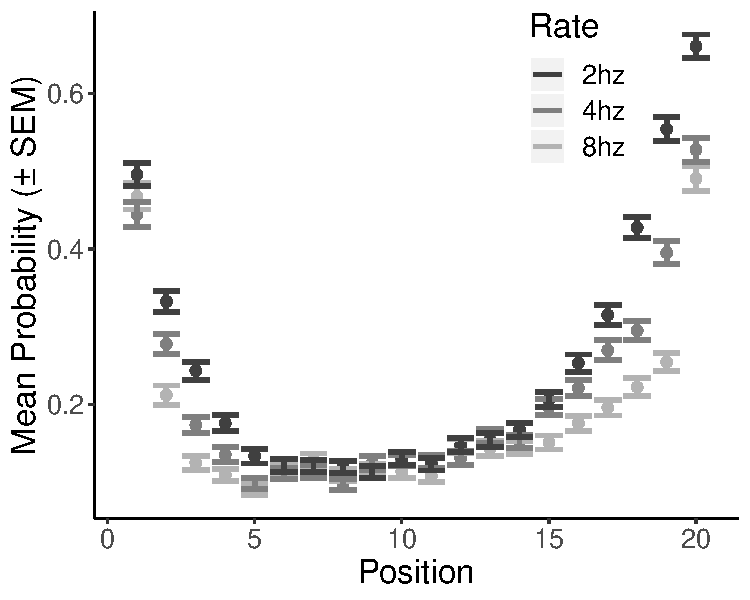
\includegraphics[width = .4\textwidth]{SPC_adjusted.pdf}
\end{center}
\caption{Probability of recall as a function of position in study list. Participants showed the highest level of performance for items at the beginning and end of the list. As presentation rate increased, participants showed a tendency to have a lower recency effect in comparison to the primacy effect} 
\label{SPC}
\end{figure}

\subsection{The Contiguity Effect Flattens At Higher Presentation Rates}
\begin{figure*}
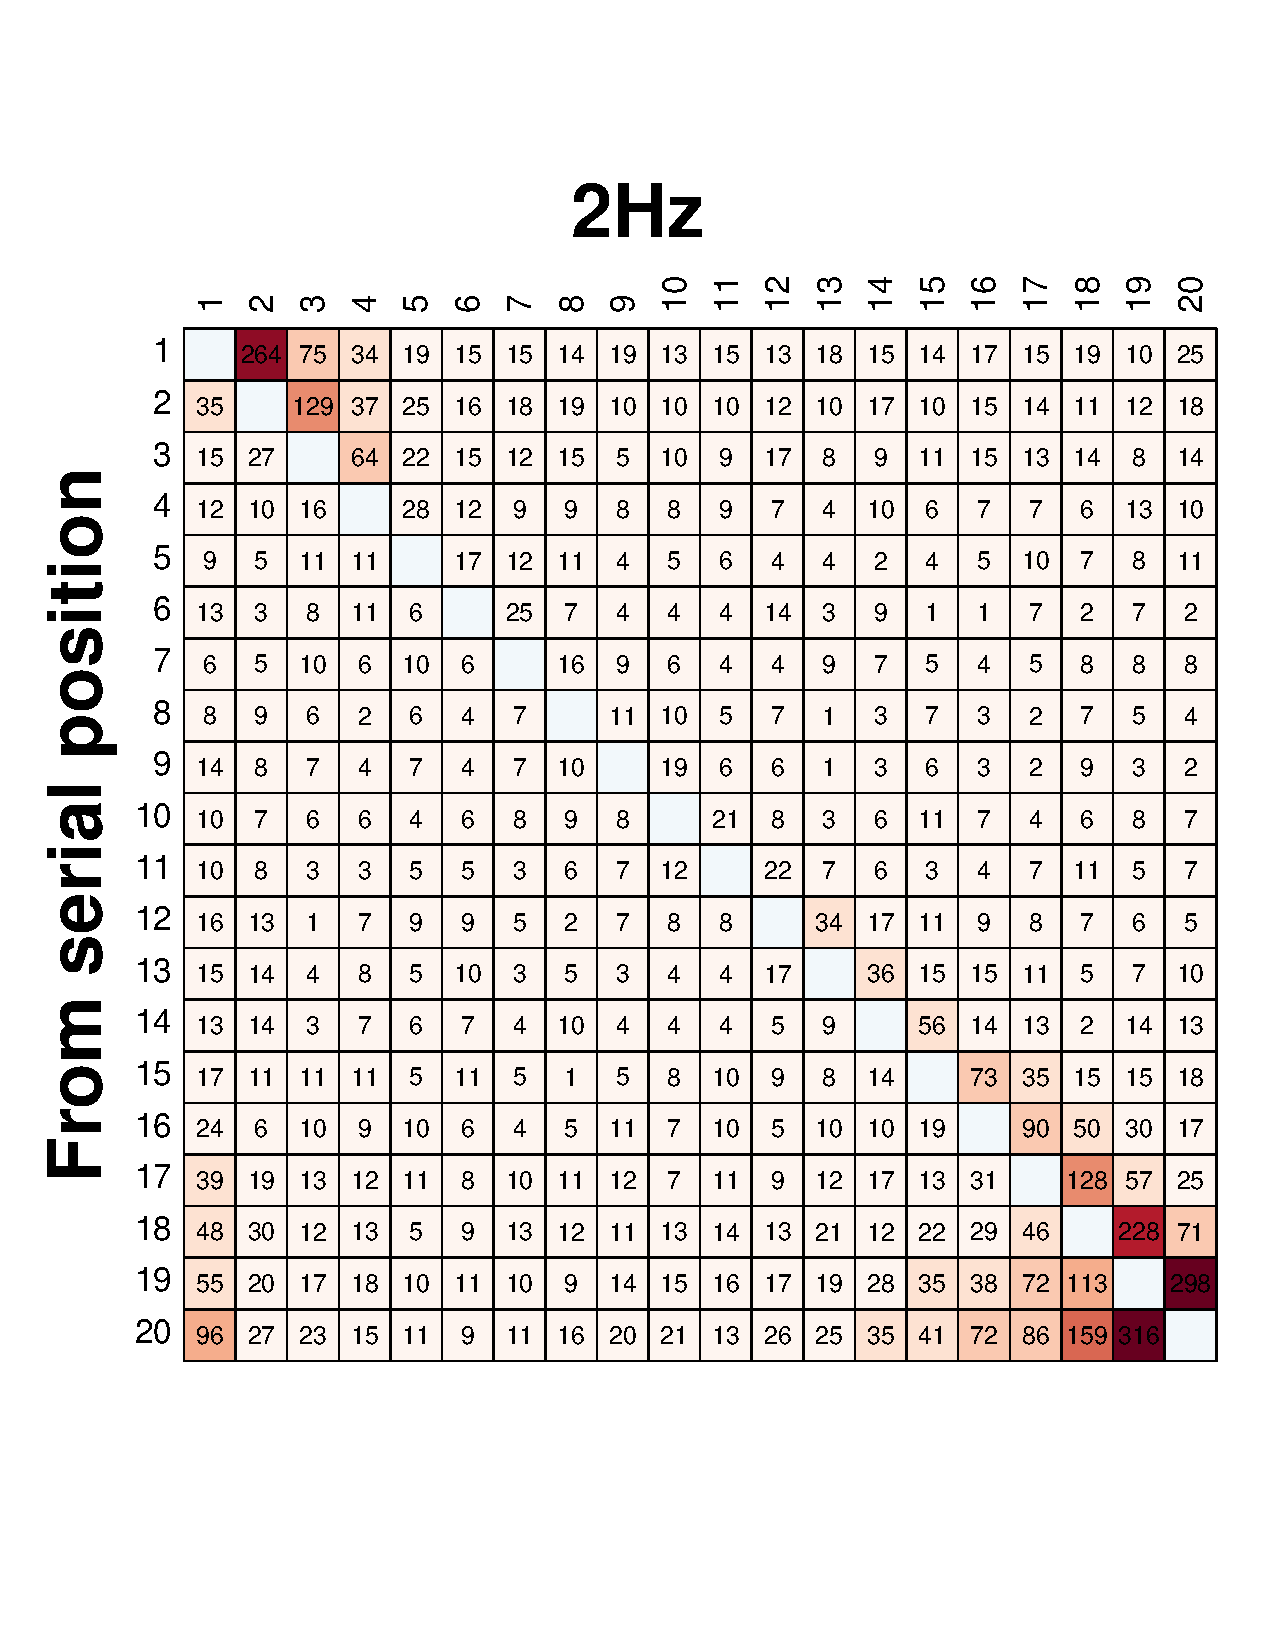
\includegraphics[width = .32\textwidth]{RSVPFR/2hz_mat.pdf}
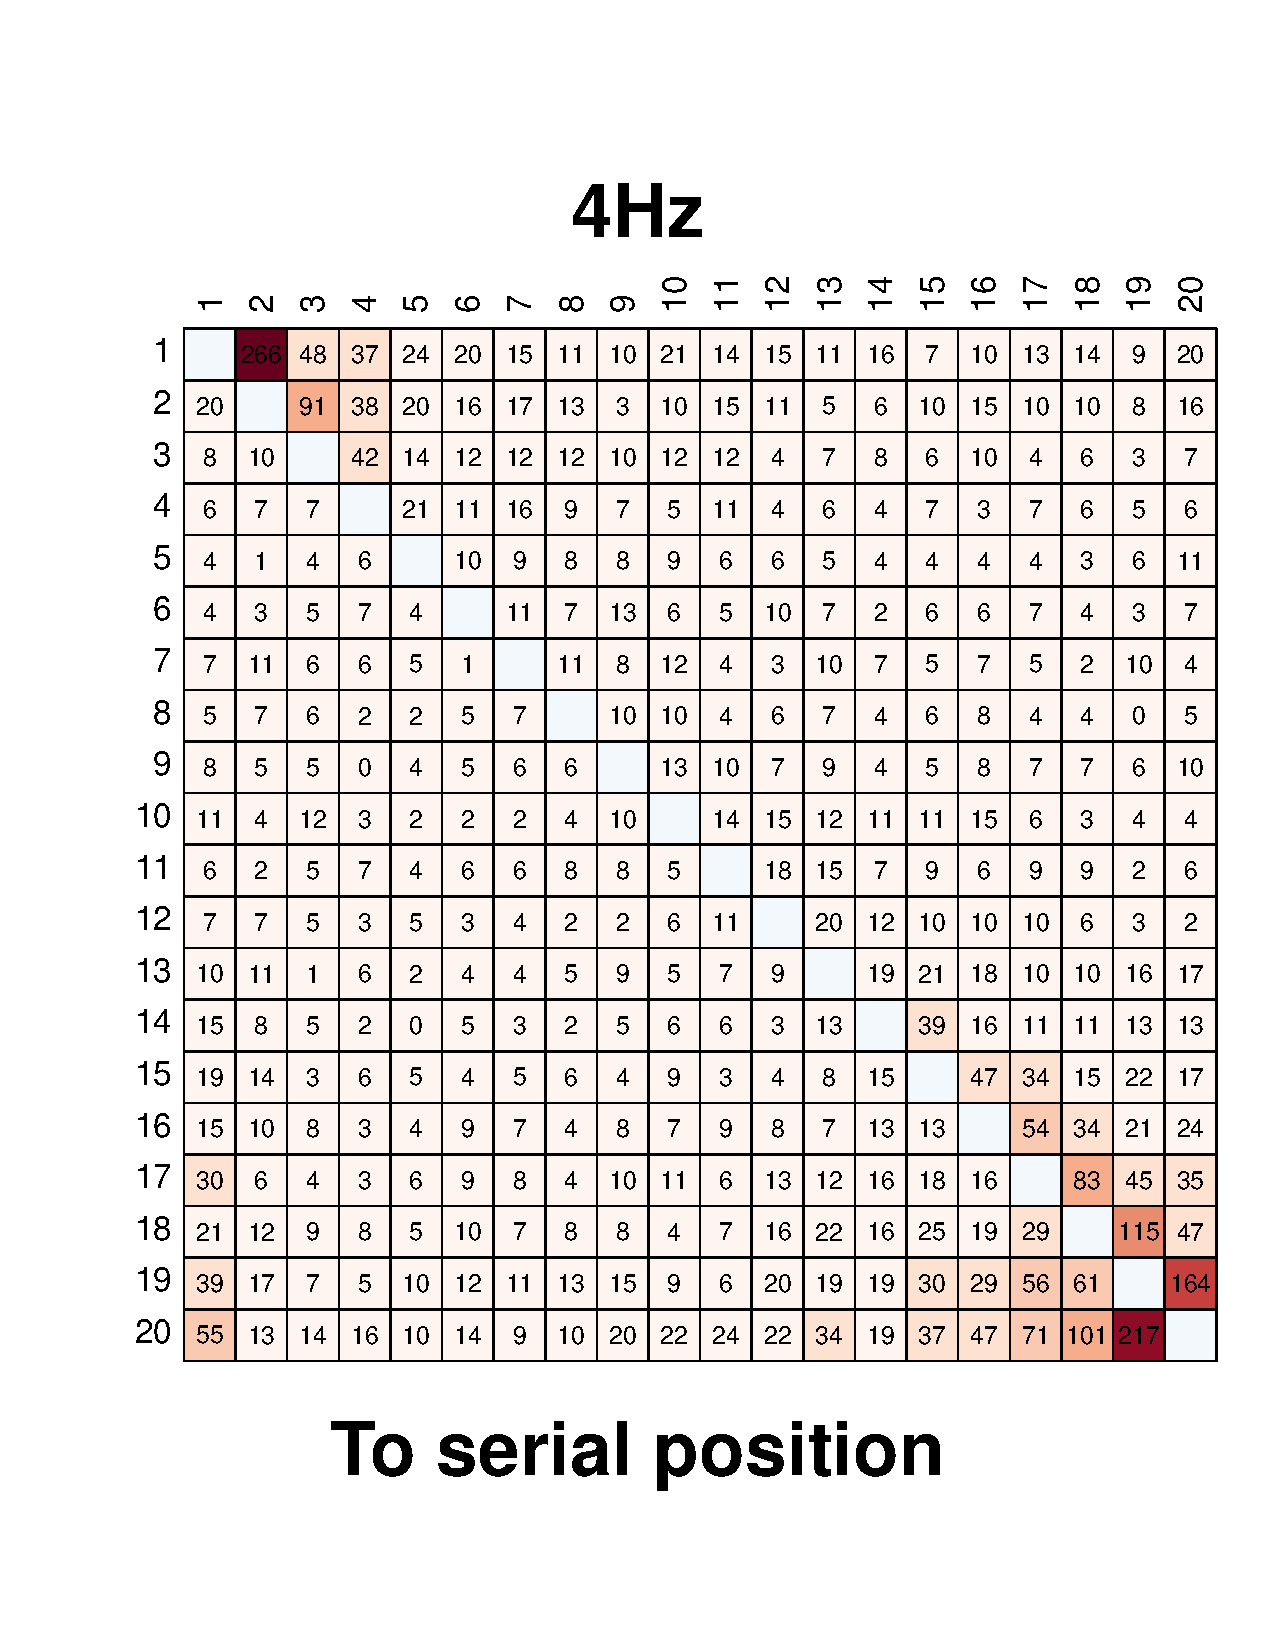
\includegraphics[width = .32\textwidth]{RSVPFR/4hz_mat.pdf}
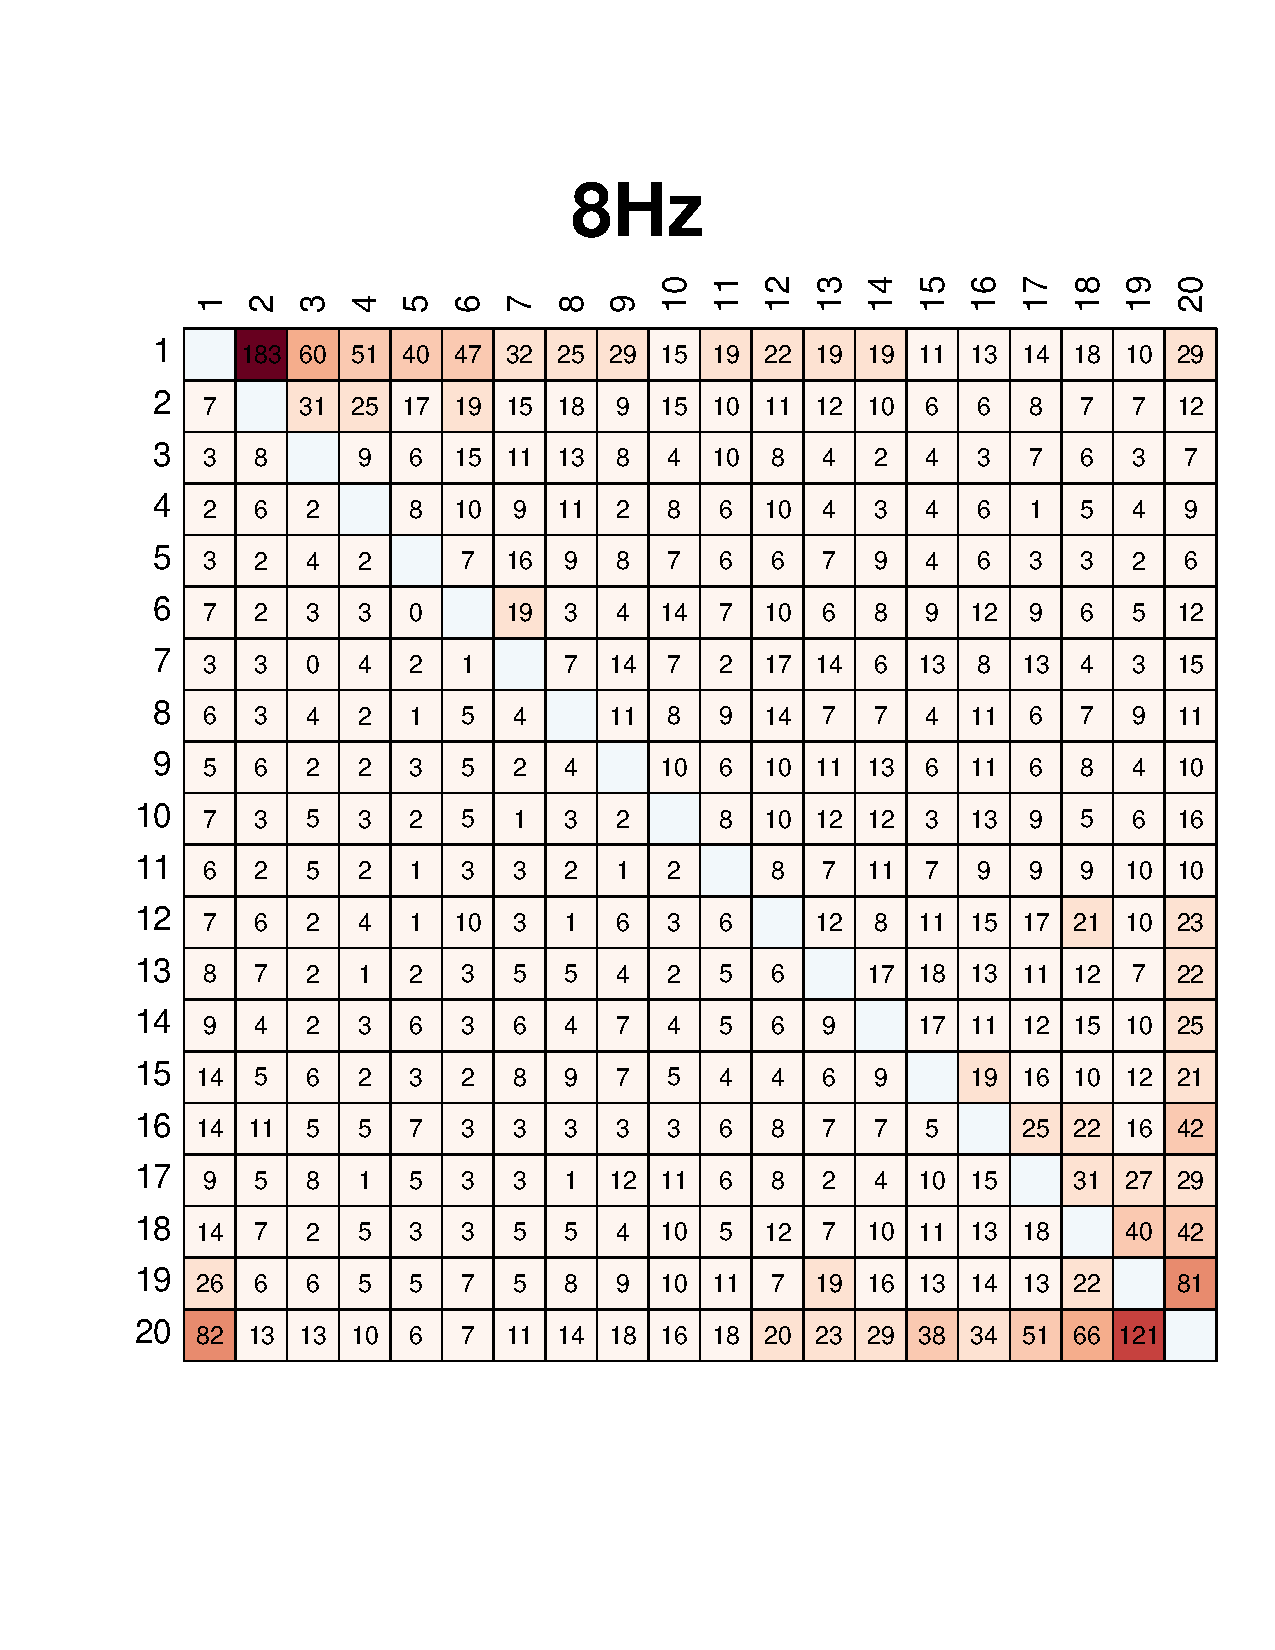
\includegraphics[width = .32\textwidth]{RSVPFR/8hz_mat.pdf}
\caption{Matrices showing the number of total valid recall transitions between
any two study list positions for each presentation rate separately. Colors and
numbers correspond to the number of such recalls summed across participants.
Transitions between extreme positions in study lists correspond to primacy and
recency effects, which persist across rates. In contrast, the likelihood of
recalling nearby items (i.e., close to the diagonal) appears to decrease as
presentation rate increases.} \label{uCRP}
\end{figure*}

Figure~\ref{uCRP} shows the number of transitions between each serial position
in each of the three conditions.  The 
primacy and recency effects can be readily distinguished, as is the tendency
to make remote transitions to the beginning of the list.
The contiguity effect can be seen as a slightly darker shade along the
diagonal; the forward asymmetry appears as a darker shade just above the
diagonal. As expected, the contiguity effect appeared to decrease as
presentation rate increased.  Because primacy and recency effects can be a
confound in identifying the contiguity effect we calculated the
lag-CRP using only transitions that came from items from the middle of the
list (serial positions 7-13).

Figure~\ref{CRP} displays the average probability of transitioning from a
recalled word to a word at a given lag (with lag~0 corresponding to
the diagonal of the matrices in Figure~4), and appears to show a reduction in
the temporal contiguity effect as the presentation rate increases. We
performed a mixed effect logistic regression to estimate the probability of
recall based on absolute lag for each presentation rate separately. This showed 
that distance from the previously-recalled item significantly decreased the probability
of recall for 2~Hz ($z=-9.74, p<0.001$) and 4~Hz ($z=-4.93, p<0.001$), but not for 8~Hz ($z=-0.70, p=0.48$).
This suggests that the contiguity effect breaks at around 8~Hz.
We then computed another mixed effects logistic regression to test 
the interaction between absolute lag, its direction (backwards
or forwards from the previously recalled item), and the presentation rate.
This analysis showed that transitions in the forward direction were more
probable than backward transitions ($z = 4.18, p<0.001$); transitions at more
distant lags were less probable ($z=-4.83, p<0.001$); probabilities were
higher for 2 Hz compared to 4 Hz ($z=-2.28, p=0.02$) and 8 Hz ($z=-3.63, p<0.001$); 
the effect of absolute lag was stronger for forward transitions than backwards transitions ($z=-2.71,
p<0.01$), and the effect of lag was stronger for 2~Hz compared to 4~Hz
($z=2.11, p=0.03$) and 8~Hz ($z=3.12, p<0.01$). All other interactions showed
no significant effects (all $p>0.05$). These results show that increasing the
presentation rate of study words has a negative effect on the temporal
contiguity effect, and nullifies it at 8~Hz.

\begin{figure}
\begin{center}
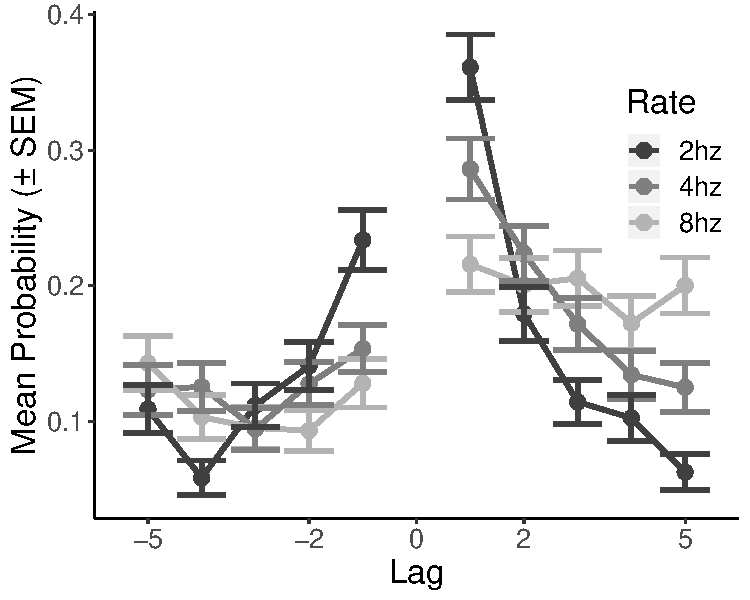
\includegraphics[width = .4\textwidth]{CRP_adjusted.pdf}
\end{center}
\caption{Lag CRP adjusted for primacy and recency effects. As presentation rates increase, the contiguity effect weakens but remains asymmetric.} 
\label{CRP}
\end{figure}

\section{Discussion}

Remembering past events is associated with a jump back in time, manifesting in
a higher probability for temporally contiguous elements to be subsequently
recalled. In this study, we investigated whether higher presentation rates
would negatively impact the temporal contiguity effect. 
Many of our results were consistent with previous free recall studies. For
instance, the average number of words recalled per list decreased as the
presentation rate increased. Also, as the presentation rate increased, the
strength of the primacy effect increased compared to the recency effect.
The novel contribution of this paper is the finding that 
the temporal contiguity effect was disrupted by fast presentation rates, most
notably in the 8~Hz condition.   These findings suggest that encoding
processes taking place on the order of 125~to~250~ms are important for binding
items to their temporal context.
%Furthermore, there was a
%pronounced asymmetry between forward and backward transition probabilities,
%consistent with a failure to build temporal associations while maintaining an
%ability to recover a previous state of contextual drift. 
% A
%novel finding was that individuals were more likely to initiate recall with
%the first item on the list in the 8~Hz condition, whereas recall of the last
%item was more likely in the other conditions. 
% Claudio: Marc highlighted something here with no comment

Our results pose questions about the relation of presentation rate and neural
coding. Medial temporal lobe theta (3-8Hz) is related to successful encoding
in free recall, particularly when binding elements temporally
\cite{NyhuCurr10,SedeEtal03}. In addition, \citeA{GudeEtal09} have shown that
prediction of successfully-recalled items relies on theta frequency. While
presentation rates of 2~Hz and 4~Hz are mostly contained within this frequency
band, 8~Hz lies at the upper bound of human theta. It is possible that
presening eight words per second outpaces encoding processes that depend on
theta \cite{HassEtal02}, thus explaining why lag CRPs become weaker for this
presentation speed. Examination of encoding and retrieval periods using EEG
and ECoG could help address this issue in the future.

\nocite{GudeEtal09}


\bibliographystyle{apacite}

\setlength{\bibleftmargin}{.125in}
\setlength{\bibindent}{-\bibleftmargin}

\bibliography{bibdesk}


\end{document}
